\documentclass[a4paper]{article}
\usepackage{fancyhdr}
\usepackage[includeheadfoot,left=1in, right=0.5in, top=0.5in, bottom=0.5in]{geometry}
\usepackage{lastpage}
\usepackage{extramarks}
\usepackage[usenames,dvipsnames]{color}
\usepackage{graphicx}
\usepackage{listings}
\usepackage{courier}
\usepackage{tikz}
\usepackage{color}
\usepackage{float}
\usepackage{url}
\usepackage{subfigure}
\usepackage{varwidth}
\usepackage{caption}
\usepackage{multirow}
\usepackage[pdfborder={0 0 0}]{hyperref}
\usepackage[compact,small]{titlesec}
\usepackage{microtype}
\usepackage{verbatim}
\usepackage{booktabs}
\usepackage{indentfirst}
\usepackage{enumitem}
\usepackage{pdfpages}

\captionsetup[sub]{labelsep=newline}

% line spacing
\linespread{1.0}

% bold item
\let\origitem\item
\renewcommand{\item}{\normalfont\origitem}
\newcommand{\bolditem}{\small\bfseries\origitem}

% tilde
%\newcommand{\small_tilde}{\raise.17ex\hbox{$\scriptstyle\sim$}}

% indent item
\newcommand{\indentitem}{\setlength\itemindent{24pt}}

% perfect tilde
\newcommand{\tildep}{\raise.17ex\hbox{$\scriptstyle\sim$}}

\parskip = 0.5\baselineskip
\setlength{\belowcaptionskip}{-\baselineskip}

\captionsetup{font=scriptsize}
\captionsetup{labelfont=bf}

\pagestyle{fancy}
\rhead{Samir Silbak \& Manasa Kasula}
\lhead{EECE6080 - Project}
\rfoot{Page\ \thepage\ of \protect\pageref{LastPage}}
\cfoot{}
\renewcommand\headrulewidth{0.4pt}
\renewcommand\footrulewidth{0.4pt}

% make verbatim text small
\makeatletter
\g@addto@macro\@verbatim\small
\makeatother

\setlength\parindent{0pt} % Removes all indentation from paragraphs
%\setlength\parindent{24pt}

\definecolor{sh_comment}{rgb}{0.12, 0.38, 0.18 } %adjusted, in Eclipse: {0.25, 0.42, 0.30 } = #3F6A4D
\definecolor{sh_keyword}{rgb}{0.37, 0.08, 0.25}  % #5F1441
\definecolor{sh_string}{rgb}{0.06, 0.10, 0.98} % #101AF9

%\sectionfont{\centering}
\lstset{
    language=vhdl,
    xleftmargin=.25in,
    xrightmargin=.25in,
    numbers=left,
    numberstyle=\tiny,
    frame=tb,
    showstringspaces=false,
    captionpos=b,
    stringstyle=\color{sh_string},
    keywordstyle = \color{sh_keyword}\bfseries,
    commentstyle=\color{sh_comment}\itshape,
    basicstyle=\small\sffamily,
    %numbersep=-5pt,
    belowskip=\baselineskip,
    aboveskip=\baselineskip
}
\usepackage{authblk}

\title{
    \vspace{2in}
    \textbf{VLSI \\}
    \vspace{10pt}
    \textbf{PROGRAMMABLE BINARY TREE COMPUTATION\\}
    \vspace{10pt}
    \textbf{CHIP NAME: PBTCKS}
    \vspace{2in}
}

\author[1]{Samir Silbak}
\author[2]{Manasa Kasula}

\affil[1]{silbaksr@mail.uc.edu}
\affil[2]{kasulama@mail.uc.edu
    \vspace{10pt}
}
\affil[1]{(513) 207-0687}
\affil[2]{(847) 612-7364
    \vspace{2.0in}
}
\titleformat*{\section}{\large\normalfont}

\begin{document}

%\includepdf{}
\maketitle
\newpage
\parskip = 0.2\baselineskip
\newpage
\tableofcontents
\newpage
\listoffigures
\listoftables
\lstlistoflistings
\parskip = 0.5\baselineskip
\newpage
\input{../progress_1/progress_1_body.tex}
\newpage
\input{../progress_2/progress_2_body.tex}
\newpage

\section{\textbf{Chip Level Layout}}

    \begin{figure}[H]
        \centering
        \includegraphics[width=\textwidth,height=\textheight,keepaspectratio]{../../magic/pics/magic_layout_32_bit.png}
        \caption{\textbf{32 Bit Layout - Magic}}
        \label{fig:gg}
    \end{figure}

    %\begin{figure}[H]
    %    \centering
    %    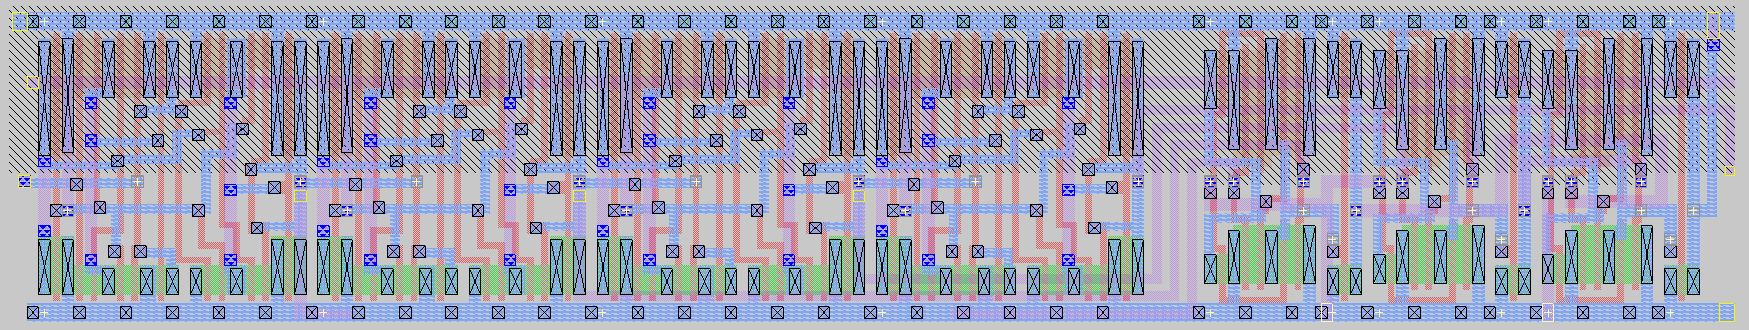
\includegraphics[width=\textwidth,height=\textheight,keepaspectratio]{../../magic/pics/lut_slice_internal.png}
    %    \caption{\textbf{LUT Slice Internal Magic Layout}}
    %    \label{fig:gg}
    %\end{figure}

\section{\textbf{Users Guide}}

    %\begin{figure}[H]
    %    \centering
    %    \includegraphics[width=\textwidth,height=\textheight,keepaspectratio]{../../docs/waveforms/normal_mode_ug.png}
    %    \caption{\textbf{Cycle Timing Diagram for Normal Mode}}
    %    \label{fig:gg}
    %\end{figure}

    \begin{figure}[H]
        \centering
        \includegraphics[width=\textwidth,height=\textheight,keepaspectratio]{../../docs/waveforms/normal_mode_ug_32.png}
        \caption{\textbf{Cycle Timing Diagram for Normal Mode}}
        \label{fig:gg}
    \end{figure}

    In normal mode, the user will need to leave the TMEI signal low. The user will then need to give data inputs
    to both PI and LI. Since, LI has 4 times the number of bits that P has, LCLK should then be triggered for
    4 times longer than PCLK. The final computation is shown to be on the very last clock cycle. Also, it does not
    matter whether the P input or LUT inputs are loaded in first, the functionality of the circuit will still remain
    working properly. Note to the user, in this timing diagram, we are showing that P input is loaded in first.

    \begin{figure}[H]
        \centering
        \includegraphics[width=\textwidth,height=\textheight,keepaspectratio]{../../docs/waveforms/test_mode_ug_32.png}
        \caption{\textbf{Cycle Timing Diagram for Test Mode Enable}}
        \label{fig:gg}
    \end{figure}

    %\begin{figure}[H]
    %    \centering
    %    \includegraphics[width=\textwidth,height=\textheight,keepaspectratio]{../../docs/waveforms/test_mode_ug.png}
    %    \caption{\textbf{Cycle Timing Diagram for Test Mode Enable}}
    %    \label{fig:gg}
    %\end{figure}

    In test mode, we are connecting all the D-Flip Flops together to make sure all the flip flops are shifting properly. This
    scheme is known as a scan chain. Here we can see that when TMEI is high, we are in test mode. The output of the last clock
    signal and data output of P will be connected to the input of the LCLK and LI, respectively. Since the architecture contains
    32 bits for the P input and 124 (31*4) bits for the LUT, we will have to shift in a vector of 156 bits (124+32) in order to
    see the output of the scan chain. Only then can the user monitor the output to verify that all the shift registers are working
    as intended. Note that F (the final computation) is not shown in this timing diagram, because the user is not concerned with
    the functionality of the LUTs in this mode--only monitoring the shift registers.

    The user will need to set TMEI high, then he/she will have to give the data inputs to PI and make sure to have a total of
    156 clock cycles for PCLK, the rest is taken care of by the hardware (the user will not have to give any inputs to the LUT).

    %In test mode, we are connecting all the D-Flip Flops together to make sure all the flip flops are shifting properly. This
    %scheme is known as a scan chain. Here we can see that when TMEI is high, we are in test mode. The output of the last clock
    %signal and data output of P will be connected to the input of the LCLK and LI, respectively. Since the architecture contains
    %64 bits for the P input and 252 (63*4) bits for the LUT, we will have to shift in a vector of 316 bits (252+64) in order to
    %see the output of the scan chain. Only then can the user monitor the output to verify that all the shift registers are working
    %as intended. Note that F (the final computation) is not shown in this timing diagram, because the user is not concerned with
    %the functionality of the LUTs in this mode--only monitoring the shift registers.

    %The user will need to set TMEI high, then he/she will have to give the data inputs to PI and make sure to have a total of
    %316 clock cycles for PCLK, the rest is taken care of by the hardware.

    %The timing diagram here illustrates how these are connected in hardware. Therefore, the last slice of P (63rd in this case) will
    %be taken into the input of the first slice of LI and will have to shift as mentioned 316 bits before seeing the first output.

\section{\textbf{Test Strategy}}
    We have a few methods for testing to ensure that the chip is working correctly. The first method we use for testing purposes
    is to connect all the D-Flip Flops together to create the initial scan chain. This will allow the user to make sure all of
    the shift registers are working properly. Another method, is to have individual bit slice designs completely independent of
    the circuit itself. Therefore, we have the Look Up Table Slice and the P-shift register slice completely independent of the
    circuit. The third method consists of having separate standard slices, both an inverter and a D-Flip Flop completely independent
    of the circuit as well. The final method consists of monitoring certain signals within each cell. Other testing strategies include
    looking at the clock output signals and making sure that the signal follows the input clock signals. If the user ensures these
    signals are not lagging, then it's safe to conclude that the signal strength provided by the buffers are sufficient enough to
    overcome the capacitance.

    In the first method, the user will only need to pull the TMEI pin high.

    In the second method, the user will need to feed the individual bit slice inputs as noted:

    \underline{LUT slice:}

    TSCI (test slice clock input) is the input to the clock line. \newline
    TSD (test slice D input) is the input to the LUT, the user will shift in the combinational function he/she desires to test. \newline
    TSA and TSB (test slice A and B) are inputs and act as the address lines into the LUT, the user should feed these inputs after
    ``programming'' the LUT. \newline
    TSQ is the output of the LUT, the user can probe this pin to make sure everything that was shifted in is correct. \newline
    F is the output of the final computation the LUT slice performs. The user can can probe this pin to monitor that \newline
    the final computation is working as intended. \newline
    TSCO (test slice clock output) is the output to the clock line.

    \underline{P Shift register Slice:}

    TSCI (test slice clock input) is the input to the clock line. \newline
    TSPI (test slice p input) is the input to the signal P. \newline
    TSPO (test slice p output) is the output signal of P.

    The third method consists of two separate standard cells, the inverter and the DFF:

    \underline{Inverter:}

    TII (test inverter input) is the input to the inverter, the user will give this pin any value. \newline
    TIO (test inverter output) is the output to the inverter, the user will probe this pin to monitor the output.

    \underline{D-Flip Flop:}

    TFCI (test flip flop clock input) is the input to the test clock line, the user will give this pin the clock signal. \newline
    TFDI (test flip flop D input) is the input to the D-Flip Flop, the user will give this pin an input value to be monitored. \newline
    TFQO (test flip flop Q output) is the output of the D-Flip Flop, the user will use this pin to monitor the output. \newline
    TFCO (test flip flop clock output) is the output of the clock line.

    For the last and final method, we have certain pins used to monitor certain various areas within the circuit. The user should
    use the Pin description to see each output pin needed to test to ensure the functionality of the circuit is performing correctly.

\section{\textbf{Descrption of Chip Architecture}}
    The PBCTKS architecture uses a 32-bit wide P register and a 124-bit wide LUT register for programming
    mode. This allows the user to program up to 2**32 different combinations for given inputs and 2**(124/4)
    different combinations to program the functionality of the chip. This chip consists of \tildep 31 I/O pins
    which include test pins for testing purposes, and includes a pin to set the chip in normal or testing mode.

    %The PBCTKS architecture uses a 64-bit wide P register and a 252-bit wide LUT register for programming
    %mode. This allows the user to program up to 2**64 different combinations for given inputs and 2**(252/4)
    %different combinations to program the functionality of the chip.
    %is designed for 64-bit

\section{\textbf{Major Design Decisions}}
    We layed everything out in magic, and noticed that we would only be using about 60\% of chip area. This was
    just unacceptable, so we needed to come up with a different layout design where we would be able utilize more
    of the chip area. We decided to design how we needed to rearrange the slices in a more compact fashion. In Figure 49,
    we can see the method of the layout that would have been used in Magic.

    Unfortunately, we were very constrained with time, and connecting the VDD and GND lines became exponentially complicated
    that we had to stop and revert back to the 32 bit design. The incomplete 64 bit design can be shown below.

    \begin{figure}[H]
        \centering
        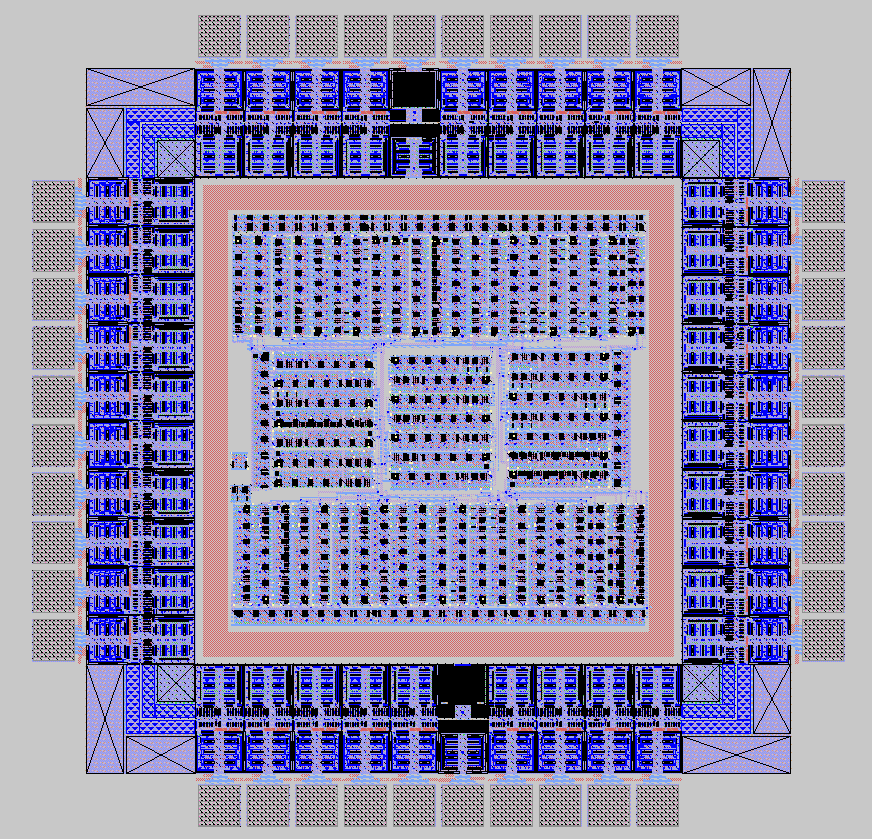
\includegraphics[width=\textwidth,height=\textheight,keepaspectratio]{../../magic/64_bit/layout/magic_layout_64.png}
        \caption{\textbf{64 Bit Layout in Magic}}
        \label{fig:gg}
    \end{figure}

    Here we can see that we maximized not only N, but the total area that was given to us. But as I have mentioned previously, due
    to wiring complexity and timing constraints, we were not able to complete this on time and had to revert back to the original
    32 bit design.

    %The figure below shows the initial magic layout, we had originally come up with. We can see here
    %not only were we not able to utilize the total area, but our N was surely not maximized. In conclusion, we
    %came up with the new design layout shown below. Even though the complexity of the wiring has not changed,
    %everything else became maximized.

    \begin{table}[H]
        \centering
        \begin{tabular}{l | l }
            \hline
            \textbf{DFFPOSX1} &  \textbf{Capacitance (pF)} \\ \hline
            \midrule
                CLK     & \tildep 0.05 \\
                D       & \tildep 0.0157 \\
        \end{tabular}
        \caption{\textbf{Capacitance Values for D-Flip-Flop}}
    \end{table}

    \begin{table}[H]
        \centering
        \begin{tabular}{l | l | l }
            \hline
            \textbf{BUFFX4} &  \textbf{Capacitance (pF)} & \textbf{Cap Output Drive Strength (pF)}\\ \hline
            \midrule
                A     & \tildep 0.0322  & 1.85\\
                Y     & \tildep 0.0322 \\
        \end{tabular}
        \caption{\textbf{Capacitance Value and Output Drive Strength for Buffer}}
    \end{table}

    Since the clock signal was global and driving all of the slices, we needed to accommodate for the capacitance. In the
    table above we can see that the capacitance of the D-Flip Flop was found to be 0.05pF. Therefore, we knew that this
    capacitance would add up over all of the bit slices, so we needed to make sure to add buffers when needed. The table above
    shows the output drive strength for the given buffer. We then used this to calculate the maximum buffers that could be used:
    1.85pF / 0.05pF \tildep 37. Therefore, we ended up just putting a buffer every 32 DFFs (leaving 5 for error).

    %\begin{table}[H]
    %    \centering
    %    \begin{tabular}{l | l }
    %        \hline
    %        \textbf{INVX1} &  \textbf{Capacitance (pF)} \\ \hline
    %        \midrule
    %            A     & \tildep 0.0161 \\
    %    \end{tabular}
    %    \caption{\textbf{Capacitance Value for Inveter}}
    %\end{table}

    %\begin{table}[H]
    %    \centering
    %    \begin{tabular}{l | l }
    %        \hline
    %        \textbf{MUX2X1} &  \textbf{Capacitance (pF)} \\ \hline
    %        \midrule
    %            A     & \tildep 0.0322 \\
    %            B     & \tildep 0.0322 \\
    %            S     & \tildep 0.0364 \\
    %    \end{tabular}
    %    \caption{\textbf{Capacitance Value for 2:1 Multiplexer}}
    %\end{table}

\section{\textbf{IRSIM Simulations}}

    \begin{figure}[H]
        \centering
        \includegraphics[width=\textwidth,height=\textheight,keepaspectratio]{../../irsim/pics/f_del.png}
        \caption{\textbf{Top Delay Normal Mode}}
        \label{fig:gg}
    \end{figure}

    We can see the worst case delay time found in IRSIM shown in the above picture. This is very consistent with
    what we have seen in our VHDL design.

    \begin{figure}[H]
        \centering
        \includegraphics[width=\textwidth,height=\textheight,keepaspectratio]{../../irsim/pics/lut_test_slice.png}
        \caption{\textbf{Test LUT Slice}}
        \label{fig:gg}
    \end{figure}

    We can see that the independent LUT slice works correctly.

    \begin{figure}[H]
        \centering
        \includegraphics[width=\textwidth,height=\textheight,keepaspectratio]{../../irsim/pics/p_test_slice.png}
        \caption{\textbf{Test P Shift Register Slice}}
        \label{fig:gg}
    \end{figure}

    We can see that the independent P Shift Register slice works correctly.

    \begin{figure}[H]
        \centering
        \includegraphics[width=\textwidth,height=\textheight,keepaspectratio]{../../irsim/pics/dff_test_slice.png}
        \caption{\textbf{Test DFF Slice}}
        \label{fig:gg}
    \end{figure}

    We can see that the independent DFF slice works correctly.

    \begin{figure}[H]
        \centering
        \includegraphics[width=\textwidth,height=\textheight,keepaspectratio]{../../irsim/pics/inv_test_slice.png}
        \caption{\textbf{Inverter}}
        \label{fig:gg}
    \end{figure}

    We can see that the independent Inverter works correctly.

\section{\textbf{VHDL Simulations}}
    \begin{figure}[H]
        \centering
        \includegraphics[width=\textwidth,height=\textheight,keepaspectratio]{../../vhdl/waveforms/top_32_nm.png}
        \caption{\textbf{Top 32-bit Normal Mode}}
        \label{fig:gg}
    \end{figure}

    \begin{figure}[H]
        \centering
        \includegraphics[width=\textwidth,height=\textheight,keepaspectratio]{../../vhdl/waveforms/top_32_tm.png}
        \caption{\textbf{Top 32-bit Test Mode}}
        \label{fig:gg}
    \end{figure}

    \begin{figure}[H]
        \centering
        \includegraphics[width=\textwidth,height=\textheight,keepaspectratio]{../../vhdl/delay_waveforms/top_del_32_nm.png}
        \caption{\textbf{Top Delay 32-bit Normal Mode}}
        \label{fig:gg}
    \end{figure}

    \begin{figure}[H]
        \centering
        \includegraphics[width=\textwidth,height=\textheight,keepaspectratio]{../../vhdl/delay_waveforms/top_del_32_tm.png}
        \caption{\textbf{Top Delay 32-bit Test Mode}}
        \label{fig:gg}
    \end{figure}

    \begin{table}[H]
        \centering
        \begin{tabular}{l | l | l }
            \hline
               & \textbf{VHDL} & \textbf{IRSIM} \\ \hline
            \midrule
                F           & 5.470 ns & 6.32 ns\\
        \end{tabular}
        \caption{\textbf{Total Delay Times for Normal Mode between VHDL and IRSIM}}
    \end{table}

    F is the final output computation for the Look Up Table (this was our worst case delay). We can see here that the times
    are fairly close to one another. Note this is the total delay, but keep in mind that the delay per slice for worst case
    delay was found to be 2.6ns. So our Maximum clock frequency is found to be 1/2.6ns, approximately 385 MHz.

    %\begin{table}[H] \centering
    %    \begin{tabular}{l | l | l | l}
    %        \hline
    %        &  \textbf{IRSIM}   & \textbf{VHDL} & \textbf{Hspice}\\ \hline
    %        \midrule
    %            Inverter    & 0.11 ns & 0.159 ns & 0.1627 ns \\
    %            Mux         & 0.315 ns & 0.312 ns &  0.31214 ns \\
    %            DFF         & 0.255 ns & 0.198 ns & 0.20305 ns \\
    %    \end{tabular}
    %    \caption{\textbf{Delay Times}}
    %\end{table}

\section{\textbf{Simulation Strategy}}
    It was much easier to use Python to write to the cmd file, and then check the output log file if anything failed.
    It would be too difficult to give a 124 bit vector manually, so we used Python to feed the signals for both in
    VHDL and IRSIM. Also, since we want to make sure things works as intended, the best method was to just shift in
    all 1's for all the DFF, and monitor the outputs accordingly. This gave us an idea if something was being shorted out
    or something was not shifting out properly. Then we monitored each node for debugging purposes to ensure that each bit
    was being shifted out from one flip flop to the next. A figure below shows the method used.

    \begin{figure}[H]
        \centering
        \includegraphics[width=\textwidth,height=\textheight,keepaspectratio]{../../irsim/pics/irsim_debug.png}
        \caption{\textbf{Debug Mode in IRSIM}}
        \label{fig:gg}
    \end{figure}

\section{\textbf{Work Division}}
    \begin{table}[H]
        \centering
        \begin{tabular}{l | p{8cm}}
            \hline
            \textbf{Student}   & \textbf{Task} \\ \hline
            \midrule
                Both        & Modified Pin-out Diagram \\
                Both        & Magic Layout \\
                Both        & IRSIM \\
                Both        & VHDL \\
                Both        & Modified Floor Plan
        \end{tabular}
        \caption{\textbf{Task Assignment}}
    \end{table}

\end{document}
